\section{Output dimension with 1,814-PC targets}\label{sec:dimension}
The earlier comparison fixes the output dimension at three. A separate
experiment asks how much of the measured error can be reduced by allowing
more coordinates. This changes the input target as well as the question:
the same 1,500 cells are extracted from the previously verified
full-population 1,814-PC matrix. Those PCs retain 99.002235 percent of the
variance of the centered, unscaled, transformed 3,290-gene matrix across
120,804 cells. The projection is not refitted for the sparse-MDS input.
Consequently these scores must not be compared directly with the earlier
20-PC scores as if their denominators were unchanged.

Here $x_i\in\mathbb R^{1814}$, the targets remain
$d_{ij}=\|x_i-x_j\|_2$, and $y_i\in\mathbb R^d$, with
\[
d\in\{3,4,5,10,20,25,50,100,200,300\}.
\]
The all-pairs score $R$ and sparse proxy are still
Equations~\eqref{eq:full} and~\eqref{eq:proxy}; every evaluation uses all
1,124,250 pairs, in original distance units and without post-fit rescaling.
The 99-percent variance threshold describes the input projection, not a
guarantee of 1-percent relative-distance error.

\subsection{Matched settings and completed fits}
All dimensions share one preparation with 200 internally selected
distance-proportional landmarks, regional endpoint counts, and symmetric
union-of-10-nearest-neighbor local interactions. The preparation seed is
20261021. For neighbor selection only, a centered, unscaled PCA fitted to
the subset retains 506 dimensions and about 90.02 percent of the subset's
1,814-PC variance. Mean retention of the ten nearest neighbors relative
to search in all 1,814 PCs is 86.37 percent, using the same intersection
definition as above. Every target distance still uses all 1,814 PCs.
The preparation contains \dimensionfittedpairs\ positive-weight pairs.

Each dimension has one start, with seed 20190619 for initialization and
fitting. A common Gaussian matrix with 300 columns supplies the first $d$
columns, which are centered and scale-fitted by the earlier formula.
These are related, nested random starts, not identical configurations:
adding coordinates and refitting the starting scale changes distances.
The SGD backend uses the same weight-dependent schedule in every dimension,
with $T=100$ and $\epsilon=0.1$ in Equation~\eqref{eq:schedule}.
These are completed 100-epoch schedules, not the first 100 epochs of the
earlier 500-epoch schedule. There is no edge-KK refinement.

Ten fits were attempted and all ten completed 100 epochs; none failed,
were skipped, or were excluded. Ten single-threaded workers were launched,
with fewer remaining active as smaller jobs finished. Peak sampled
aggregate resident memory was 4.23 GiB, below the 50 GiB watchdog threshold.
Sampling every two seconds is a monitored stop condition, not an operating
system hard cap. Per-fit native workspace allowance was 4 GiB.
All final errors were independently recomputed through Gram-matrix
distances and agreed within $10^{-8}$ percentage points. These checks
verify the scores, not convergence or a globally optimal embedding.

\begin{figure}[htbp]
\centering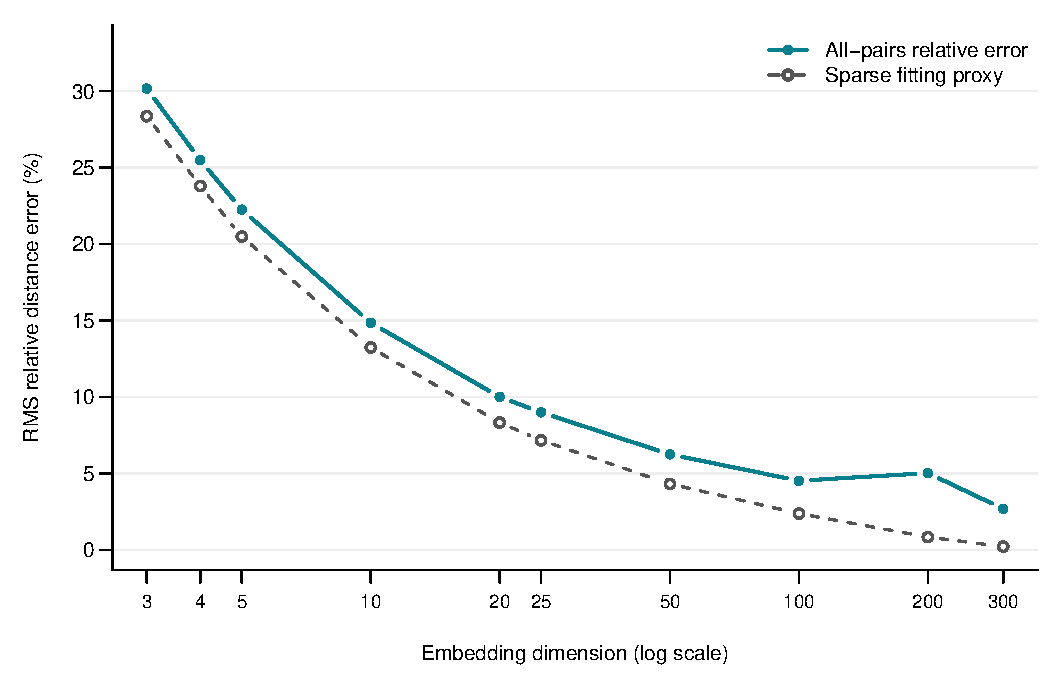
\includegraphics[width=\linewidth]{dimension-error.pdf}
\caption{Error after 100 SGD epochs versus output dimension for the same
1,500 cells and shared 200-landmark preparation. Filled teal points show
all-pairs RMS relative error; open gray points show the sparse proxy.
The horizontal axis is logarithmic; connecting segments guide the eye
between tested dimensions, not a fitted response curve. The all-pairs
error decreases substantially overall, but increases from 100D to 200D
even though the proxy continues to fall. No uncertainty band is available
from the single start per dimension.}
\label{fig:dimension}
\end{figure}

The all-pairs error falls from 30.164 percent in 3D to 10.000 percent in
20D and 2.680 percent in 300D. This is a substantial gain in reproducing
the chosen ambient distances, not evidence that biological geometry has
300 intrinsic dimensions. Dimensional restriction, the sparse approximation,
initialization and finite optimization all contribute to the achieved error.
In particular, the 200D score of 5.017 percent is higher than the 100D
score of 4.516 percent, despite a lower proxy (0.832 versus 2.371 percent).

\begin{table}[htbp]
\centering\begin{tabular}{rrr}\toprule
$d$ & All-pairs RMS (\%) & Sparse proxy RMS (\%) \\ \midrule
3 & 30.164 & 28.357 \\
4 & 25.483 & 23.791 \\
5 & 22.246 & 20.486 \\
10 & 14.850 & 13.230 \\
20 & 10.000 & 8.324 \\
25 & 8.987 & 7.158 \\
50 & 6.242 & 4.309 \\
100 & 4.516 & 2.371 \\
200 & 5.017 & 0.832 \\
300 & 2.680 & 0.210 \\
\bottomrule\end{tabular}

\caption{Terminal 100-epoch results on the 1,814-PC targets. $d$ is output
dimension; the all-pairs column is $R$ in Equation~\eqref{eq:full}, and
the proxy column is $100\sqrt{S_{\rm proxy}}$. Both are RMS percentages
but use different pair weights and denominators. Values are individual
fits, not means; one start per dimension does not support an uncertainty
interval. Lower values indicate closer distance agreement under the
respective score.}
\label{tab:dimension}
\end{table}
\FloatBarrier

\subsection{Where the 200D excess error occurs}
The proxy and the all-pairs score differ in two ways: which pairs contribute
directly, and how those pairs are weighted. To separate these effects,
let $F=\{\{i,j\}\in E:c_{ij}>0\}$ be the set of directly fitted pairs,
and let $U$ contain the remaining unordered pairs. Write $m_F=|F|$,
$m_U=|U|$, and $f=m_F/M$. Define the \emph{unweighted} RMS relative
error within each set by
\begin{equation}
R_A=100\sqrt{\frac{1}{|A|}\sum_{\{i,j\}\in A}
\left(\frac{r_{ij}-d_{ij}}{d_{ij}}\right)^2},\qquad A\in\{F,U\}.
\end{equation}
These scores give each pair equal weight within its own set. In contrast,
the proxy weights pairs in $F$ by $c_{ij}$. Since $F$ and $U$ partition
all pairs, their exact relationship to the overall score is
\begin{equation}\label{eq:partition}
R^2=fR_F^2+(1-f)R_U^2.
\end{equation}
Thus squared RMS percentages, not RMS percentages themselves, combine
linearly with the pair fractions.

There are $m_F=\dimensionfittedpairs$ directly fitted pairs
($\dimensionfittedfraction$ percent of all pairs) and
$m_U=\dimensionomittedpairs$ remaining pairs (74.18 percent).
The sets and weights are identical for the 100D and 200D fits.

\begin{table}[htbp]
\centering\begin{tabular}{rrrrr}\toprule
$d$ & $R$ & $R_F$ & $R_U$ & Proxy \\ \midrule
100 & 4.516 & 2.545 & 5.023 & 2.371 \\
200 & 5.017 & 0.896 & 5.801 & 0.832 \\
\bottomrule\end{tabular}

\caption{A diagnostic decomposition of the saved final fits, with no
rerunning of optimization. All numeric scores are RMS percentages.
$R$ evaluates all pairs equally; $R_F$ evaluates directly fitted pairs
equally; $R_U$ evaluates pairs absent from the fitting list equally.
``Proxy'' uses the regional endpoint-average weights on $F$.
The table isolates pair selection from reweighting within $F$.}
\label{tab:partition}
\end{table}
\FloatBarrier

The 200D fit improves agreement on the directly fitted pairs even without
their proxy weights: $R_F$ falls from 2.545 to 0.896 percent.
However, $R_U$ rises from 5.023 to 5.801 percent. Because $U$ contains
nearly three quarters of all pairs, its deterioration outweighs the
improvement on $F$ in Equation~\eqref{eq:partition}. This is the measured
reason for the higher overall RMS score. The discrepancy is not merely
a different normalization of two otherwise identical errors, nor only
reweighting within the fitting set.

Pairs in $U$ are not directly penalized by the sparse proxy, although their
distances can be influenced indirectly through shared cells, landmarks
and regional counts. They are not a statistically independent test set:
the same cells and input geometry helped construct the preparation and
the starting scale. The decomposition describes distance reconstruction,
not prediction on new cells.

Higher dimension itself cannot force a worse best attainable all-pairs
score. Appending 100 zero columns to a 100D configuration gives a feasible
200D configuration with exactly the same distances. Therefore
\begin{equation}
\inf_{Y\in\mathbb R^{1500\times200}}S_{\rm rel}(Y)
\ \leq\
\inf_{Y\in\mathbb R^{1500\times100}}S_{\rm rel}(Y).
\end{equation}
This statement concerns the best attainable score, not the terminal
configuration produced by a particular sparse-SGD run. The 200D run
reaches a configuration with better selected-pair agreement but worse
agreement elsewhere. Additional degrees of freedom, different starts,
and finite optimization can permit such outcomes; this experiment does
not isolate their separate contributions or establish that either fit
is trapped in a local minimum.

The 300D trace illustrates the same distinction over time: from epoch 10
to epoch 100 its proxy falls from 0.7724 to 0.2099 percent while its
all-pairs error rises slightly from 2.6183 to 2.6801 percent.
Useful diagnostics would repeat starts, increase landmark coverage, and
test a 200D warm start formed from the 100D result plus small nonzero extra
coordinates. Exactly zero extra coordinates alone would preserve the
lower-dimensional span under ordinary noncoincident pair updates.
Such diagnostics would be separate experiments, not replacements for
the results reported here.
